%%%%%%%%%%%%%%%%%%%%%%%%%%%%%%%%%%%%%%%%%%%%%%%%%%%%%
\documentclass[apj]{emulateapj}
%\documentclass[preprint2]{aastex61}
%\documentclass[12pt,preprint]{aastex}
\graphicspath{{figures/}}
\DeclareGraphicsExtensions{.jpg,.pdf,.png,.eps,.ps}

%\usepackage[table,usenames,dvipsnames]{xcolor}
%\usepackage{amsmath}
%\usepackage{subfigure}
\usepackage[backref,breaklinks,colorlinks,citecolor=blue]{hyperref}
\usepackage{natbib}
%\usepackage{natbib}
\bibliographystyle{fapj}
%\usepackage{graphicx}
%\usepackage{multirow}

\newcommand{\sqdeg}{deg$^2$ }
\newcommand{\omb}{\ensuremath{\Omega_b h^2}}
\newcommand{\omc}{\ensuremath{\Omega_c h^2}}
\newcommand{\clpp}{\ensuremath{C_{L}^{\phi\phi}}}
\newcommand{\cpmf}{\ensuremath{C_{\ell}^{\rm pmf}}}
\newcommand{\apmf}{\ensuremath{A_{\rm pmf}}}
\newcommand{\bpmf}{\ensuremath{B_{\rm 1\,Mpc}}}
\newcommand{\alens}{\ensuremath{A_{\rm lens}}}
\newcommand{\lcdm}{\ensuremath{\Lambda}CDM}
\newcommand{\nrun}{\ensuremath{n_{\rm run}}}
\newcommand{\neff}{\ensuremath{N_{\rm eff}}}
\newcommand{\ho}{H\ensuremath{_0}}
\newcommand{\mnu}{\ensuremath{\sum m_\nu}}
\newcommand{\ukarcmin}{\ensuremath{\mu}K-arcmin}
\newcommand{\lknee}{\ensuremath{\ell_{\rm knee}}}
\newcommand{\fermilat}{\textit{Fermi}-LAT}

\newcommand{\be}{\begin{equation}}
\newcommand{\ee}{\end{equation}}
\newcommand{\planck}{{\sl Planck}}
\newcommand{\wmap}{{\sl WMAP}}
\newcommand{\bicepkeck}{BICEP2/Keck Array}
\newcommand{\sptnew}{SPT-3G}
\newcommand{\pb}{POLARBEAR}
\newcommand{\simons}{Simons Array}
\newcommand{\sptpol}{SPTpol}
\newcommand{\advactpol}{Adv.~ACTpol}

\newcommand{\tbd}[1]{\textcolor{Red}{{\bf TBD}: #1}}
\newcommand{\gab}[1]{\textcolor{Orchid}{[{\bf GS}: #1]}}

%

% ref to section \S\ref{sec:label}

%\submitjournal{ApJ}
\def\Melbourne{1}
\def\uci{2}
%%%%%%%%%%%%%%%%%%%%%%%%%%%%%%%%%%%%%%%%%%%%%%%%%%%%%
\begin{document}

\title{Current and future constraints on primordial magnetic fields}
\author{D.~Sutton\altaffilmark{\Melbourne}, C.~Feng\altaffilmark{\uci}, and C.~L.~Reichardt\altaffilmark{\Melbourne}}
\altaffiltext{\Melbourne}{School of Physics, University of Melbourne, Parkville, VIC 3010, Australia}
\altaffiltext{\uci}{Department of Physics and Astronomy, University of California, Irvine, CA 92697-4575, USA}
\email{christian.reichardt@unimelb.edu.au}

\begin{abstract}

We present new limits on the amplitude of potential primordial magnetic fields (PMFs) using temperature and polarization measurements of the cosmic microwave background (CMB)  from \planck{}, \bicepkeck{}, \pb, and \sptpol. 
We reduce twofold the upper limit on the CMB anisotropy power due to a PMF, from $\apmf < 0.73$ from Planck alone to $\apmf < 0.35$ for the combined dataset at 95\% CL. 
%Most of the improvement is due to the addition of the \bicepkeck{} data; without these bandpowers, the combined limit weakens to $\apmf < 0.\tbd{XX}$. 
We also forecast the expected future limits from soon-to-deploy CMB experiments (like \sptnew{},  \advactpol, or the \simons) and the proposed CMB-S4 experiment. 
Future CMB experiments should dramatically reduce the current uncertainties, by two orders of magnitude for the near-term experiments and three orders of magnitude for the CMB-S4 experiment. 
The constraints from CMB-S4 have the potential to rule out much of the parameter space for PMFs.

\end{abstract}

\keywords{dark energy --- cosmic background radiation --- early universe }
\section{Introduction}
\label{sec:intro}

Measurements of the cosmic microwave background (CMB) temperature anisotropy have provided some of the most powerful tests of cosmology. 
We are now entering a new era as experiments begin to measure  polarized ``B-modes" in the CMB for the first time \citep{hanson13,polarbear14b,bicep14a,naess14,keisler15,bicepkeck15,louis16}. 
Precision measurements of CMB polarization promise new tests of the standard cosmological model. 
The best known of these tests are the searches for inflationary gravitational waves in B-modes at large angular scales and plans to measure the sum of the neutrino masses through the lensing B-modes on small angular scales \citep[for a recent review see,][]{abazajian16}. 

CMB B-mode measurements can also be used to constrain more exotic models, such as the possible existence of cosmic birefringence \citep{carroll98,lue99} or a primordial magnetic field (PMF) \citep{kosowsky96, seshadri01}.  
Both effects lead to the rotation of E-modes into B-modes. 
By equating the magnitude of the resulting B-modes, parity-violating processes can be translated into an equivalent PMF strength. 
We will therefore simply quote effective limits on a PMF. 
In this work, we present new upper limits from current CMB polarization data on the possibility of a PMF or parity-violating physics. 

Magnetic fields are ubiquitous in astronomy and are found almost universally in collapsed objects from stars to galaxies and galaxy clusters \citep[for review, see][]{ryu12, widrow12}. 
There is even some evidence for magnetic fields in intergalactic space from \fermilat{} data \citep{neronov10}, although alternative explanations \citep{broderick12} have been proposed. 
High energy $\gamma$-rays from blazars should  produce electron-positron pairs when the $\gamma$-rays collide with IR or optical photons. 
These pairs should later annihilate in at GeV energies, but the expected GeV flux is missing in the \fermilat{} observations. 
The missing flux could be explained by the deflection of particles due to intergalactic magnetic fields. 
If this is indeed the case then the GeV results set lower limits on the intergalactic magnetic field strength of $10^{-9} - 10^{-6}$\,nG \citep{tavecchio10,taylor11,dermer11,vovk12}. 

The mechanism to create large-scale magnetic fields, especially in intergalactic space, remains unclear. 
One popular proposal is that the observed fields are the product of primordial magnetic fields, which are predicted by several theories of the early Universe \citep[e.g.,][]{turner88, grasso98,ichiki06}. 
Adiabatic compression and turbulent shocks during later structure formation amplify these initial seed fields into the stronger fields observed today. 
Of course, this amplification process may have a different initial seed; other ideas include AGN or galactic dynamos \citep[for a review, see][]{giovannini04}. 
However, the possibility of PMFs opens up the intriguing idea that observations of large-scale magnetic fields may offer insights into the physics of the very early Universe. 


PMFs would have observational consequences for Big Bang nucleosynthesis \citep[e.g.,][]{kahniashvili10}, large scale structure \citep[e.g.,][]{battaner97}, the ionization history of the Universe \citep{kunze15}, and the black body spectrum of the CMB \citep[e.g.,][]{kunze14},  as well as the CMB anisotropies. 
The CMB anisotropies have yielded some of the strongest constraints on PMFs and are the focus of this work.
There have been two recent results of note. 
\citet{planck15-19} have used the \planck{} 2015 release of temperature and polarization data to set limits on a variety of PMF models. 
With the CMB power spectrum data that will be the focus of this paper, \citet{planck15-19} find 95\% CL upper limits ranging from $\bpmf < 5.6$\,nG to $<0.7$\,nG depending on the exact model. 
Here \bpmf{} is the rms field strength on a 1\,Mpc length scale. 
The \pb{} collaboration also recently announced limits on PMFs from the \pb{} data using either a 4-point estimator or B-mode power spectrum measurement in \citep{polarbear15}. 
The strongest constraints were from the B-mode spectrum; the observed upper limit was $\bpmf < 3.9$\,nG. 
Two other experiments, \sptpol{} and \bicepkeck{}, have reported B-mode power spectrum measurements recently \citep{keisler15,bicepkeck15}.
In this paper, we will combine the data from all four experiments to determine simple limits on the PMF, and then examine Fisher matrix forecasts on PMF models from the stage-III and stage-IV CMB experiments being built or designed right now. 



The outline of the paper is as follows. 
In \S\ref{sec:data}, we lay out the data used and the MCMC implementation used to constrain the PMF amplitude. 
We present the results of this analysis on current data in \S\ref{sec:results}. 
The assumed parameters for future experiments and the resulting Fisher matrix forecasts are described in \S\ref{sec:forecasts}. 
We conclude in \S\ref{sec:conclusions}. 

\section{Data and Methods}
\label{sec:data}

We use  Markov chain Monte Carlo (MCMC) methods to study constraints on PMFs. 
In this section, we first describe the CMB temperature and polarization anisotropy data used, and then discuss the MCMC implementation. 




\subsection{Data}

We use a compendium of current measurements of the CMB temperature and polarization anisotropies from ground-based and satellite experiments. 
We use \planck{} data from the 2015 release to constrain the TT, TE, EE and lensing power spectra. 
Specifically, these are the ``plik\_dx11dr21\_HM\_v18\_TT", ``lowTEB" and ``lensing" \planck{} likelihood modules. 


In addition to the \planck{} data, we use a number of recent CMB B-mode polarization measurements. 
First, we include measurements of the TE, EE and BB power spectra from the \sptpol{} experiment \citep{crites15,keisler15}. 
The BB bandpowers cover the angular multipoles $\ell \in [500,2000]$. 
We also add the BB bandpowers from \pb{} that cover the multipoles from 500 to 2500 \citep{polarbear15}. 
At these angular scales, both the \sptpol{} and \pb{} bandpowers primarily constrain the vector modes of a PMF. 
Finally, we include the latest BICEP2 and Keck Array  joint analysis \citep{bicepkeck15}. 
This latter dataset also places limits on the tensor modes of a PMF due to its coverage of lower multipoles. 
During the writing of this work, ACTpol polarization power spectra became available \citep{naess14,louis16}. 
We have not included them as the public likelihoods do not include the B-mode power spectrum; we do not expect adding the ACTpol bandpowers to significantly change the PMF limits based on a visual comparison of the current BB bandpowers from different experiments (see Fig.~\ref{fig:pmf-experiments}).
In all chains, we marginalize over the recommended foreground models for each data set. 
We do not however require consistency between these foreground models since the data don't have identical flux cuts for extragalactic sources and so on. 
In the case of an upper limit this treatment is conservative since wider foreground priors should only weaken the limit on the PMF strength. 
These data are plotted against the expected B-mode power spectrum for the standard cosmological model in Fig.~\ref{fig:pmf-experiments}. 

\subsection{Methods}

We use MCMC methods to determine the parameter constraints reported in this work. 
The results are calculated using  the {\textsc CosmoMC}\footnote{http://cosmologist.info/cosmomc (July 2015 version)} package \citep{lewis02b}. 
CosmoMC invokes  CAMB\footnote{http://camb.info}  \citep{lewis00} to calculate the CMB power spectrum for each set of cosmological parameters. 
Although CosmoMC and CAMB have a partial implementation of PMF, we choose to adopt a simpler, fast template-based calculation for the PMF power. 
We have adapted CosmoMC to add a scaled version of the template to all four CMB power spectra: TT, TE, EE, and BB, where the scale factor is \apmf. 
\be
C_\ell = C_\ell (CAMB) + \apmf \cpmf
\ee
The calculation of the PMF template, \cpmf, is described in \S\ref{sec:template}. 
Note that no other effect of the PMF is considered; this is one reason we only consider CMB data.

For the real data, unless noted, we assume the six parameter spatially flat \lcdm{} model with a single massive neutrino of 60\,meV and a seventh parameter \apmf{} describing the power due to the PMF. 
We adopt flat priors on all parameters. 
In particular, note that this is a flat prior on the observed PMF power, $\apmf$, not the rms magnetic field strength, \bpmf, that has often been used in the literature. 
In many chains, we also add \alens{} as a simple way of marginalizing over uncertainty in the predicted lensed BB power spectrum for any extension to the \lcdm{} model. 
Finally, in some cases, we allow non-zero tensors, parameterized by the tensor-to-scalar ratio, r. 

\subsection{Primordial Magnetic Field Template}
\label{sec:template}

The density and stress perturbations introduced by PMFs give rise to vorticity and gravitational waves in the early photon-baryon  plasma, i.e. vector and tensor modes, as well as scalar modes. 
The exact amplitude of these modes can be calculated by modifying the normal Boltzmann equations to includes sources due to the PMFs. 
We use the CMBACT code\footnote{\url{http://www.sfu.ca/~levon/cmbact.html}} \citep{pogosian99}  to do this calculation. 
The PMF anisotropy is assumed to be drawn from a Gaussian distribution with a power law power spectrum, $A_b k^{n_b}$. 
Here $n_b$ is the spectral index of PMF and $A_b$ is its amplitude. 
We can translate the amplitude, $A_b$, into more physically-motivated units by calculating the rms of the PMF field strength over a length scale of 1\rm{Mpc}, thereby defining $B_{\rm{1Mpc}}$. 
Finally, the timing of when the PMFs are generated matters because the PMF-induced stress anisotropy can be compensated by decoupled or partially-decoupled neutrinos. 
The timing is typically parametrized by the ratio of the scale factors at neutrino decoupling and PMF generation, $a_{\nu}/a_{\rm{PMF}}$. 

Given that we are still in the era of upper limits,  we do not explore the full 3-dimensional PMF parameter space in this work. 
Instead, we use CMBACT to calculate a PMF template for the CMB TT, TE, EE and BB power spectra at fixed parameters: $B_{\rm{1Mpc}}$=2.5 \rm{nG}, $n_b$=-2.9 and $a_{\nu}/a_{\rm{PMF}}=10^9$. 
This template includes tensor and vector PMF contributions; scalar contributions are not implemented in the code. 
We expect the missing scalar power to degrade the \planck-only results in this work.
However the missing scalar power should be  unimportant for the EE and BB spectra that are driving the tightest constraints. 
This template is plotted against other signals in the CMB B-mode power spectrum in Fig.~\ref{fig:pmf-bb}. 
We fit for a new scaling parameter, $A_{pmf}$, that rescales the PMF power spectrum template. 
We can translate the amplitude constraint on this template to a constraint on the rms magnetic field strength on 1\,Mpc scales, \bpmf, using the expected scaling:
\be
\apmf \propto \bpmf^4.
\ee
Note that the power in the tensor modes also depends on the timing of PMF generation relative to neutrino decoupling, which is not captured in the above expression. 
An unfortunate consequence of this steep fourth-power scaling is that substantial reductions in the observationally allowed vector-mode power lead to only modestly better limits on the magnetic field strength. 
However, if a PMF is detected, this same steep scaling would allow excellent constraints on its properties.

\begin{figure*}[htb]\centering
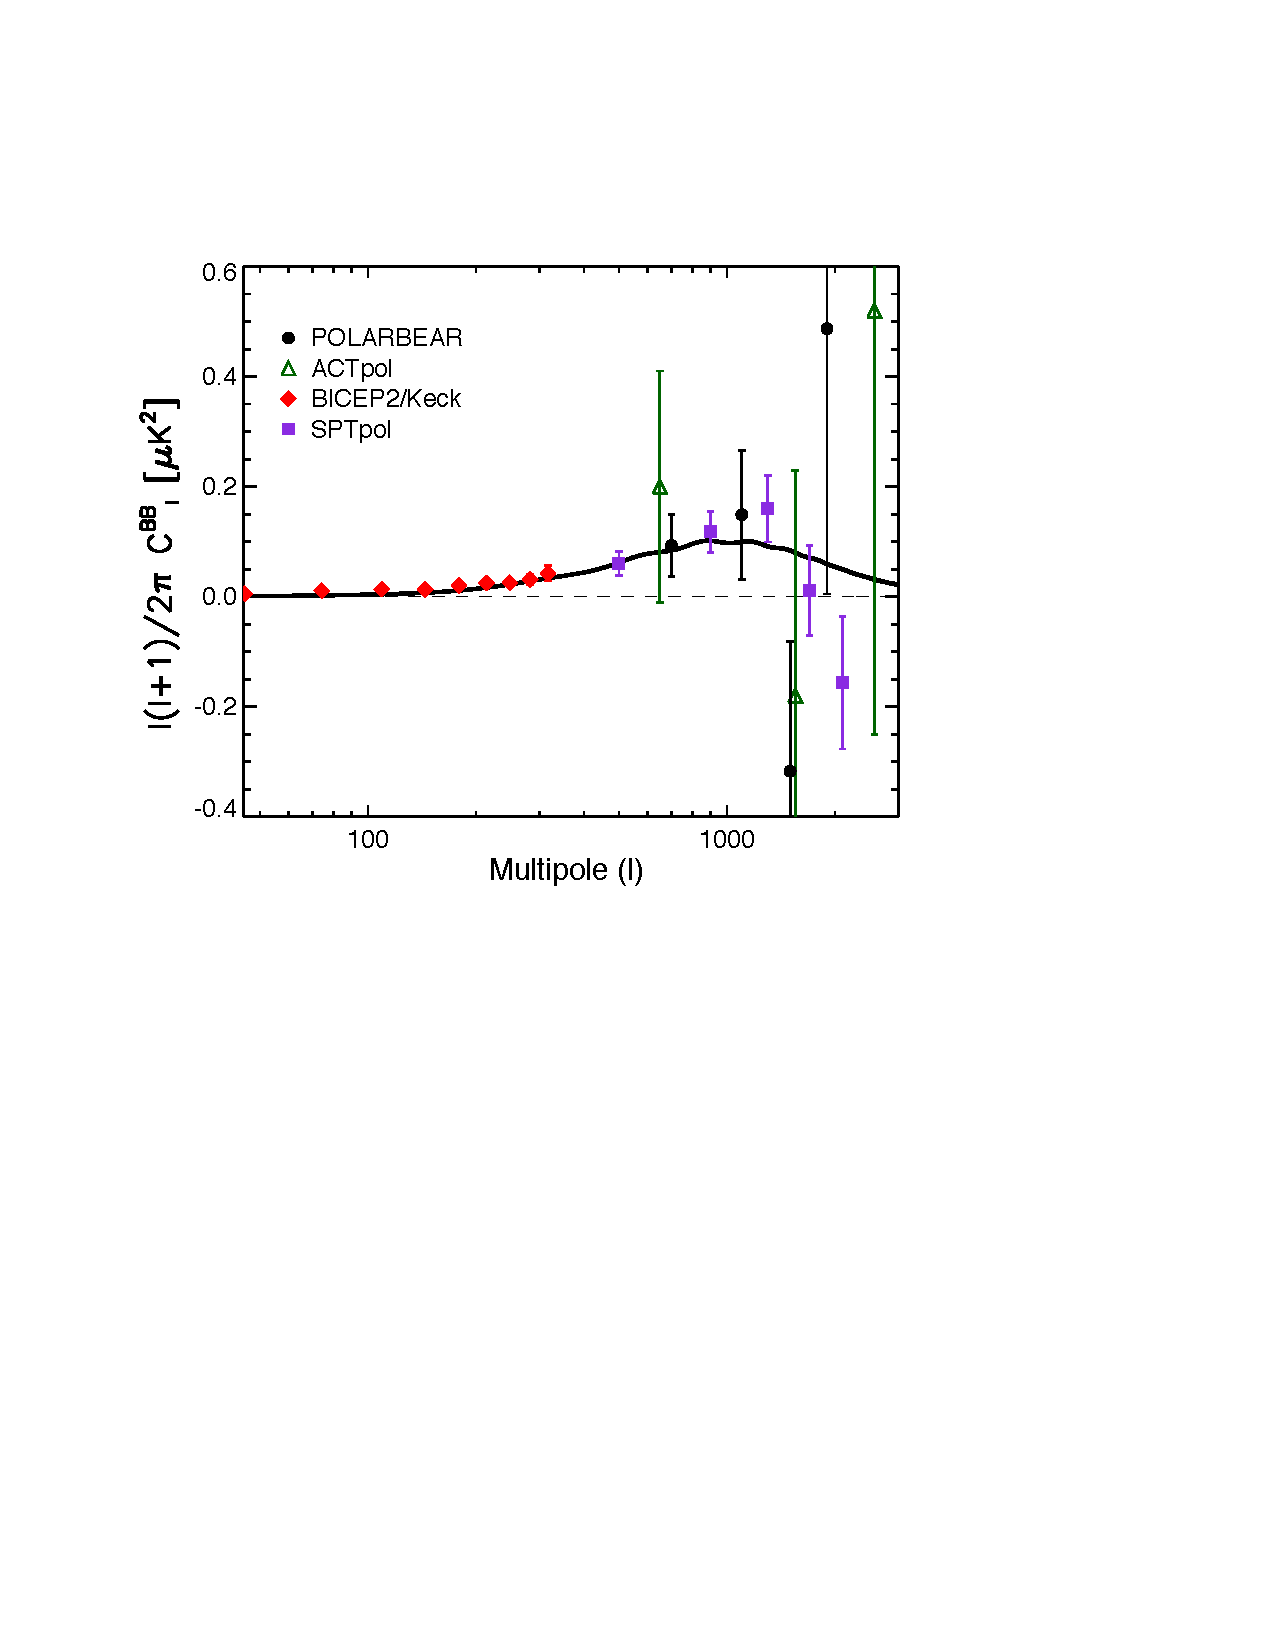
\includegraphics[width=0.9\textwidth,clip,trim={1.5cm 12.5cm 5cm 3.8cm}]{pmf_experiments.pdf}
  \caption[Current measurements of CMB B-modes]{
  Current measurements of CMB B-modes. 
    The black line shows the expected B-mode power in the \planck{} best-fit \lcdm{} cosmology (with the tensor-to-scalar ratio, r set to 0.01). 
    The B-mode measurements used for the limits in this work are denoted with filled circles; data not used has an open circle. 
    The data sets are from POLARBEAR (black; \citet{polarbear14b}); ACTpol (dark green; \citet{naess14});  BICEP2/Keck Array (red; \citet{bicepkeck15}); and SPTpol (purple; \citet{keisler15}). 
      Current B-mode measurements are noise-limited at all angular multipoles; the next generation of experiments is expected to significantly increase the signal-to-noise on the B-mode power spectrum. 
           \label{fig:pmf-experiments}
  }
\end{figure*}

\begin{figure*}[htb]\centering
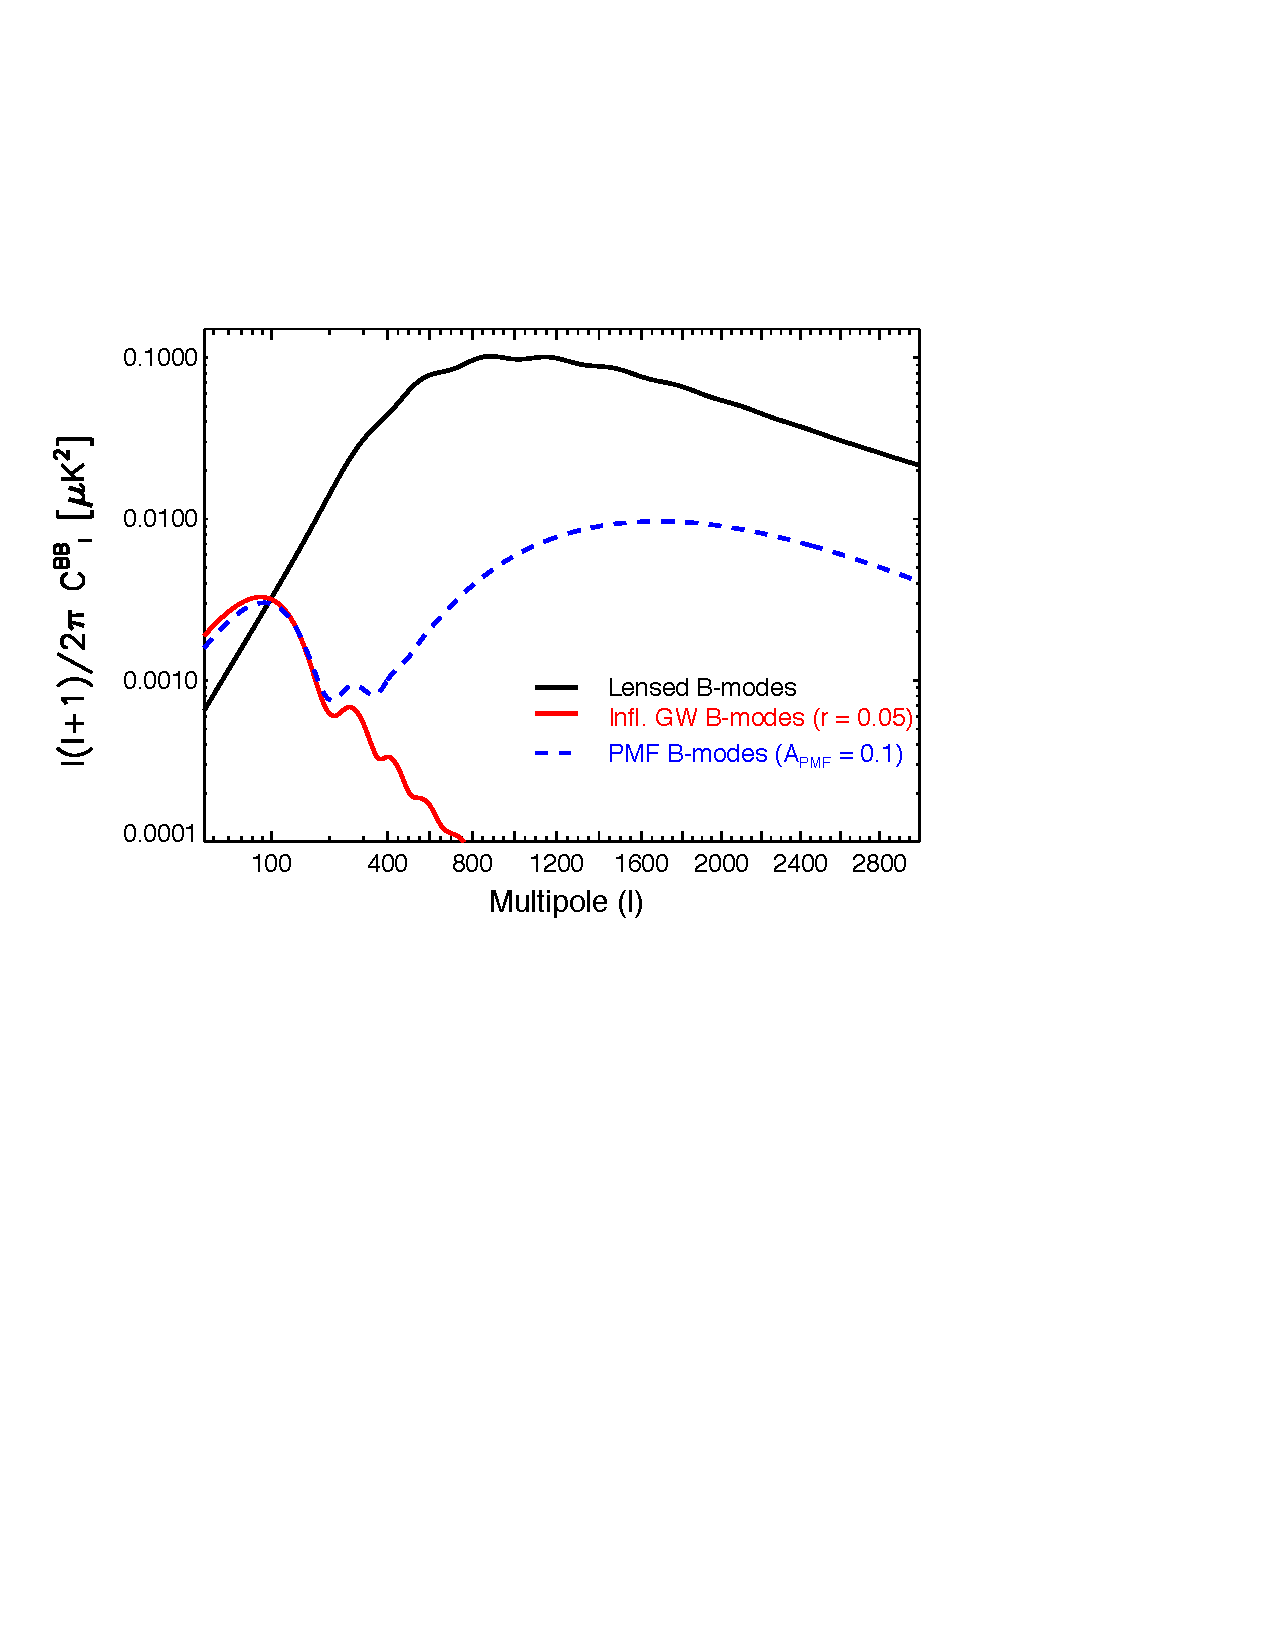
\includegraphics[width=0.9\textwidth,clip,trim={1.5cm 12.cm 5cm 4cm}]{pmf_templates.pdf}
  \caption[CMB polarization from PMFs]{
  The expected contributions to CMB B-modes. 
  The red line shows the expected lensing B-mode power in the \planck{} best-fit \lcdm{} cosmology. 
  The dark green line corresponds to the contribution from inflationary gravitational waves for $r=0.05$; the solid black line is the sum of the inflationary gravitational wave and lensing B-modes. 
  The dashed purple line shows the PMF template used in this work, scaled to \apmf{} = 0.2 to match the gravitational wave signal. 
  As can be seen, the tensor contribution from PMFs at large angular scales (low $\ell$) closely resembles the expected inflationary gravitational wave signal, and the two signals are effectively degenerate in a power spectrum (2-point) analysis.
  %However, if excess power on these scales is detected, higher order moments of the map (i.e.~4-point estimators) might be used to discriminate between   the inflationary and PMF explanations. 
      \label{fig:pmf-bb}
  }
\end{figure*}
 
\section{Results}
\label{sec:results}

We find the addition of ground-based CMB polarization data to \planck{} data substantially improves the upper limits on the allowed power due to a PMF, leading to a factor of two improvement. 
With Planck alone, the 95\% confidence upper limit is $\apmf <  0.73$ for \lcdm{}+\apmf{}; with the ground-based experiments, this limit drops to $\apmf <  0.35$. 
We list the limits for the combined dataset  with different parameter sets in Table~\ref{tab:param_all}. 
Somewhat counterintuitively, the limits are slightly better with \alens{} allowed to vary (this is due to a preference for \alens{} above unity). 
In this case for  Planck alone, the 95\% confidence upper limit is $\apmf <  0.68$, dropping to $\apmf <  0.27$ with the ground-based experiments. 
We test which datasets are important by adding single datasets to the \planck{} set while allowing \alens{} to float, and find that the majority of this improvement is due to the \bicepkeck{} ($\apmf <  0.28$) and \sptpol{} ($\apmf <  0.42$) B-mode power spectrum measurements. 
The other datasets do not have a large impact on the observed limits. 
In short, the reduction in the allowed upper limit on \apmf{} is primarily due to a more accurate measurement of the B-mode power spectrum at large angular scales. 



We propagate these limits on the observed PMF power into limits on the magnetic field strength, \bpmf. 
We assume the scaling appropriate to the vector modes, i.e. $\apmf \propto \bpmf^4$,  applies to both vector and tensor modes. 
Given this assumed scaling, the observed upper limits with a flat prior on \apmf{} would lead to an apparent `detection' of \bpmf. 
We therefore importance sample the chains to generate a flat prior on \bpmf. 
We find a 95\% limit of $\bpmf < 2.0$\,nG for \planck{} alone, completely consistent with \citep{planck15-19} who found $\bpmf < 2.0$\,nG with $n_B=-2.9$ held fixed as we've done. 
This is only slightly reduced to $\bpmf < 1.9$\,nG for the combined dataset. 
The improvement from adding more data is somewhat less than one might predict because the combined likelihood peaks somewhat above zero, whereas the \planck{}-only constraints peaks at zero. 
We also stress that this should not be treated as a robust limit as the tensor PMF modes are crucial to the improvement, and the assumed scaling has not been tested for the tensor PMF. 
We quote it nonetheless to illustrate that with a steep power law scaling, the relative improvement to \bpmf{} will be slower than the improvement to \apmf{} as more data is added.














\begin{table}[tbh]
\begin{center}
\caption{\label{tab:param_all} Parameter Constraints}
\small
\begin{tabular}{l | c c c }
Model   & $A_{pmf}$ &$A_{lens}$&$r$\\
\hline
\lcdm{} + \apmf{} &  $< 0.35$ & - & - \\
~~~+\alens{} & $< 0.27$ &$ 1.131 \pm  0.061$ &  -\\
~~~+\alens{}+r&  $< 0.24$&$ 1.133 \pm  0.062$ & $<0.056$\\ 
\end{tabular}
\tablecomments{ 
In the minimal model, \lcdm{} + \apmf{}, current CMB power spectra data from \planck, POLARBEAR, SPTpol, and \bicepkeck{} place a 95\% CL upper limit on the PMF power of $\apmf < 0.35$. 
This limit tightens slightly if tensor modes are allowed (r), or the amount of lensing is allowed to vary. 
In the case of r, the tightening is because the observed power at large angular scales is now split between PMFs or inflationary gravitational waves. 
In the case of \alens, it is because the preferred value for \alens{} is modestly above the predicted value of unity. 
Recall that the the PMF template is normalized to unity for \bpmf{} = 2.5\,nG.
} \normalsize
\end{center}
\end{table}


\section{Forecasts}
\label{sec:forecasts}

The sensitivity of CMB experiments is increasing rapidly due to the exponential growth in detector counts. 
\citet{abazajian16} thus defines four stages of CMB experiments. 
The current experiments (i.e.~the ones used for PMF constraints in the last section) are classified as Stage II experiments. 
Stage III experiments such as SPT-3G, the Simons Array, or AdvACTPol \citep{benson14,suzuki16,henderson16} have approximately ten times more detectors, and generically will start collecting data in 2017 and finish in 2020-21.
In this section, we forecast the expected constraints from EE and BB power spectrum measurements  of the Stage III experiments by combining forecasts for SPT-3G and the Simons Array. 
There is also a proposal to build a stage IV experiment, CMB-S4,  that would increase the detector counts by another order of magnitude and hopefully begin taking data in the early 2020s.
We examine the likely PMF constraints from the EE and BB power spectrum measurements with CMB-S4, and consider which aspects of experimental or survey design are important to maximize the recovered information on PMFs.




\subsection{Methods and Experimental Parameters}

We use Fisher matrices to forecast the constraints on PMFs possible from each generation of experiment. 
The Fisher matrix, $\mathcal{F}_{ij}$, can be defined as:
\be
\mathcal{F}_{ij} = \frac{1}{2} \frac{\partial^2 \chi^2}{\partial p_i \partial p_j},
\ee
for parameters, p. 
The inverse of the Fisher matrix will be the covariance matrix for the parameters. 
While Fisher matrices underestimate the true uncertainties for non-Gaussian likelihoods \citep[see e.g.,][]{wolz12}, they 
 make it easy to combine different experiments and estimate the final parameter constraints. 
 


We include two external datasets in all forecasts. 
The first dataset is the expected measurements of the  TT, TE and EE spectra from the \planck{} satellite. 
We include \planck{} TT information in the multipole range $2\le \ell \le 3000$. 
Due to the importance of galactic foreground removal at large scales in polarization, we only use TE and EE information starting from $\ell = 30$. 
A prior on the optical depth of 0.005 is added to account for the expected optical depth constraint from the missing multipoles. 
Second, we include a 1\% external measurement of the Hubble constant, such as is expected from the Taipan experiment \citep{kuehn14}. 

One concern with combining Fisher matrices from different experiments is double-counting modes due to overlapping sky coverage. 
We avoid this problem in different ways in each of the CMB power spectra. 
For the TT and TE spectra, we avoid double-counting by only using the \planck{} measurements. 
We do not expect the future experiments to substantially improve upon \planck{} in these spectra which are already cosmic variance limited out to fairly high multipoles. 
We do the opposite for the EE and BB spectra. 
We do not include \planck{} BB information in any forecast, and  we throw away \planck{} EE data in the overlap region by appropriately increasing the forecasted \planck{} EE uncertainties. 
%The exact increase depends on the assumed stage III or IV survey area.
We ignore overlaps between the stage III  with the note that the sky overlap between a Chilean experiment like the Simons Array and South Pole experiment like SPT-3G should be small. 
The overlapping sky coverage will probably be substantial between stage III and IV experiments, thus we do not include the stage III experiments, except as a prior on the polarized Poisson power, in the CMB-S4 constraints. 
With these measures, no modes should be double-counted in this analysis. 

\begin{table*}[tbh]
\begin{center}
\caption{\label{tab:experiments} Assumed survey parameters}
\small
\begin{tabular}{l || c c c c c }
Experiment & Sky coverage & Polarized Noise level  & 1/f knee & Beam FWHM \\
& &($\mu$K-arcmin)&&(arcmin.)\\
\hline
Stage III: & & & & \\

~~~~SPT-3G & 6\% & 3.0 & 200 & 1.2 \\
~~~~Simons Array & 36\% & 9.5 & 200 & 3.5 \\ 
\\
%\hline
CMB Stage IV & 55\% & 1.3 & 100 & 4.0 \\
\end{tabular}
\tablecomments{ 
Key numbers about the planned stage III and IV experiments. 
The sky coverage percentages are after galactic cuts. 
Unless otherwise noted,  the Fisher matrix forecasts in this work use these numbers. 
All forecasts also include beam and calibration uncertainties as noted in the text. 
} \normalsize
\end{center}
\end{table*}


We list the assumed survey areas, noise levels and beam sizes for each experiment in Table~\ref{tab:experiments}. 
We  assume a 5\% uncertainty on the beam FWHM and a 1\% power calibration uncertainty; we have tested relaxing or tightening the beam and calibration uncertainty and find these calibration terms have a negligible impact on the PMF constraints. 


We consider the constraints on PMFs in two cosmologies. 
The first is a 11-parameter model that extends \lcdm{} with 5 commonly considered extensions:  \lcdm{}  +r + \nrun{} + \neff{} + \mnu{}+ \apmf. 
This 11-parameter model is our default cosmological model for forecasting PMF constraints. 
We have examined the degree to which \apmf{} is degenerate with the other 10 parameters -- the only strong degeneracy is with the tensor-to-scalar ratio, r. 
The reason for this degeneracy is illustrated in Fig.~\ref{fig:pmf-bb}, which shows that the tensor mode power due to inflationary gravitational waves and PMFs is nearly identical. 
To illustrate the degree to which parameter degeneracies limit the inferred constraints,  we also quote constraints from a `minimal' 7-parameter model in which the PMF power is the only extension to \lcdm{}:  \lcdm{}  + \apmf. 
In both cases, we also marginalize over unknown Poisson EE and BB  terms due to polarized extragalactic sources. 


In this work, we only forecast the uncertainties due to power spectrum (i.e.~2-point estimators) searches for PMFs. 
Currently the power spectrum limits from \planck{} or \pb{} are better than the 4-point upper limits. 
Although outside the scope of this work, it would be interesting to extend this analysis to 4-point estimators for several reasons. 
First, the 4-point limits should improve faster as the noise level falls. 
Second, in the case of a detection, the 4-point estimators would almost certainly come into play to learn more about the vector modes of the PMFs. 
The detection (or non-detection) of the vector PMF signal in the 4-point estimators could also be used to argue for whether it is more likely that any observed tensor power is due to  inflationary gravitational waves or  PMFs. 
Finally, a lensing estimator might be used to `de-lense' the B-mode power spectrum, thereby suppressing the lensed B-mode signal and allowing better limits on PMFs. 
Such de-lensing techniques have long been proposed for inflationary gravitational wave searches \citep[e.g.][]{knox02,kesden02,seljak04a,simard15} and more recently been demonstrated on real \planck{} data \citep{larsen16}. 

%As a sanity check, we look at the Fisher matrix forecasts for Planck alone as well in both of these cases. 
%For both chains,  we look at the sigma in MCMC with \apmf{} allowed to go negative. 
%While a negative \apmf{} is unphysical, this insulates the analysis against the data preferring negative values, and thereby producing tighter limits. 
%We find for \lcdm{}  + \apmf{}: $\sigma(\apmf) = XX$ (to be compared to YY from the Fisher matrix). 
%We find for the 11-parameter model: $\sigma(\apmf) = XX$ (to be compared to YY from the Fisher matrix). 
%This degree of consistency is reasonable. \tbd{}

\subsection{Stage III forecasts}

The experiments that will begin taking data in 2017 will dramatically improve constraints on the PMF power. 
With the minimal cosmological model, the 1-sigma forecasts for \planck{}+\ho{} is $\sigma(\apmf)=0.47$ (this is consistent with, although slightly worse than, the upper limits from the real data).  
Adding the EE and BB bandpowers from the two stage III experiments (\sptnew{} and \simons{}) reduces the uncertainty nearly 400-fold in this 7-parameter model to $\sigma(\apmf)=0.0012$. 
Including all eleven parameters marginally weakens the \planck+\ho{} constraints on \apmf{} by 23\%, and the stage III constraint by a substantial factor of 2.5. 
Even within the 11-parameter model however,  the addition of stage III CMB experiments improves the \apmf{} uncertainty by a factor of $\sim$\,180 to  $\sigma(\apmf)=0.0031$. 
We can expect substantially tighter constraints on PMFs by the end of the decade. 

\subsection{Stage IV forecasts}

The primary motivation behind the proposed CMB stage IV experiment commonly called CMB-S4 is to search for inflationary gravitational waves and neutrino masses, however, the experiment should also enable extremely sensitive searches for PMFs. 
We look at the prospects for these searches using the polarization information (EE and BB power spectra) from CMB-S4. 
We begin by making forecasts for the fiducial CMB-S4 configuration as laid out in Table~\ref{tab:experiments}, and then consider how changing the experimental design would impact the expected uncertainties. 




\subsection{Survey considerations for Stage IV}

Given that CMB-S4 is still being designed, it is worthwhile to consider how design decisions will affect the final PMF constraints. 
We look at four aspects of the experiment design: the telescope size or beam FWHM, the low-$\ell$ noise performance (1/f knee),  the choice of survey area, and how well the beam size and calibration must be known. 
Of these four, we find that the low-$\ell$ noise performance and survey area are important to searches for PMFs.

Larger telescopes will allow CMB polarization to be measured on smaller angular scales, and should therefore always improve the PMF constraints. 
However, larger telescopes are also more expensive to build which means at fixed cost, they would necessitate less ambitious focal planes and lower instantaneous mapping speed. 
We find the gains due to resolution at fixed mapping speed to be negligible: a beam size of FWHM=1$^\prime$ yields only a 1\% better limit than a FWHM of 10$^\prime$. 
This illustrates how important the large angular scales are to the PMF limits. 
We very crudely approximated a cost-neutral setup with a noise level of 1.3 \ukarcmin{} for a FWHM of 4$^\prime$; a noise level of 2.9 \ukarcmin{} for a FWHM of 2$^\prime$; and a noise level of 4.1 \ukarcmin{} for a FWHM of 1$^\prime$. 
In this quasi-cost-neutral setup, there is a strong preference to go for more detectors over better angular resolution: the uncertainty was a factor of 2.5 times smaller in the coarse case over the FWHM=1$^\prime$ case. 
Raw sensitivity is more important than angular resolution to an experiment's ability to study PMFs.

\begin{figure}[htb]\centering
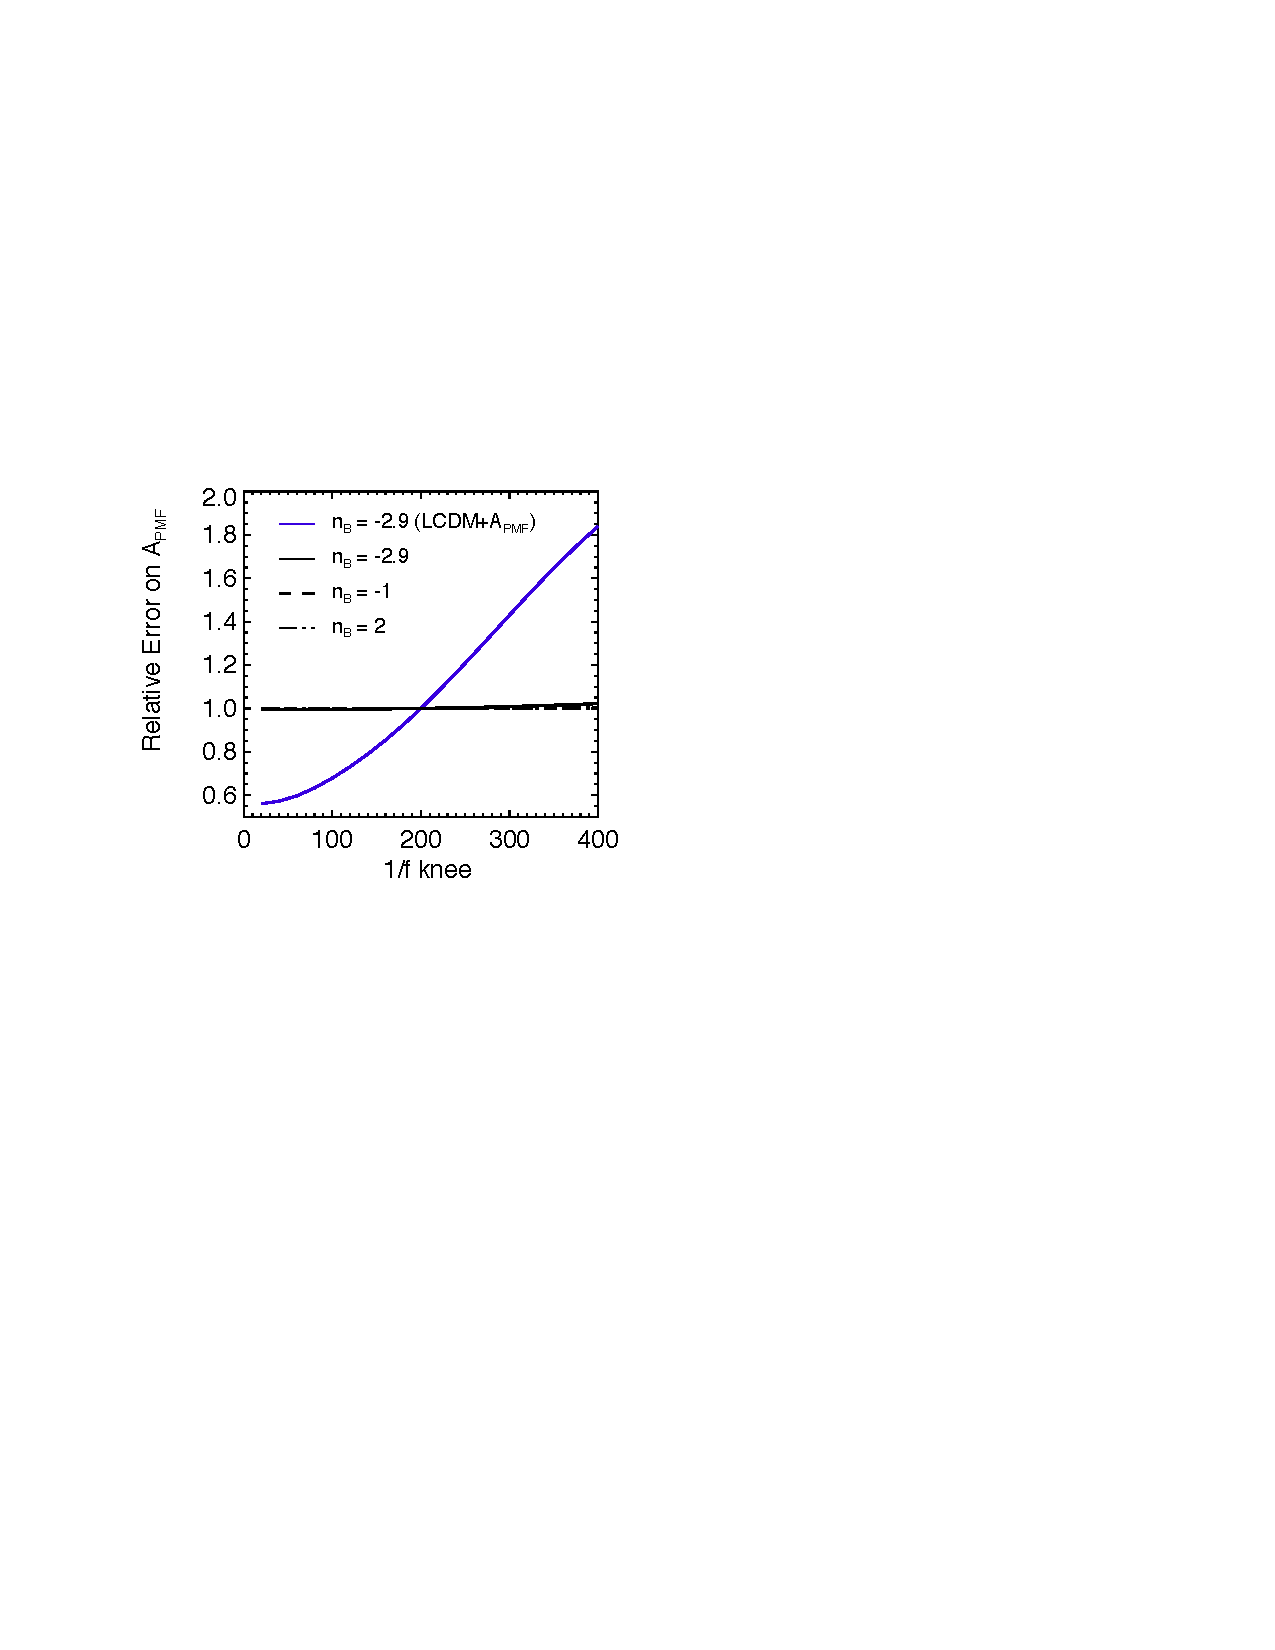
\includegraphics[width=0.45\textwidth,clip,trim={1.5cm 12.5cm 11cm 7.5cm}]{pmf_knee.pdf}
  \caption[Map knee dependence]{
  The forecasted uncertainty on the PMF power, \apmf{}, falls as expected as the low-frequency map noise decreases.  
  In particular, achieving a map 1/f knee frequency at or below $\ell = 200$ substantially improves the potential power of CMB-S4 PMF searches. 
  The black solid line shows the forecast uncertainty as a function of area in the 11-parameter cosmological model.
  The purple dot-dash line shows the same, except in the restricted \lcdm{}+\apmf{} 7-parameter model. 
  The x-axis is the map noise knee (see eqn.~\ref{eqn:knee}) in angular multipoles $\ell$. 
  As we expect, reducing low-frequency noise would lead to better PMF constraints. 
    \label{fig:knee}
  }
\end{figure}

Next we turn to the recovery of large angular scales, and the noise performance at low frequencies. 
We look at the impact of shifting the 1/f knee of the map-space noise. 
Effectively, we are multiplying the noise power, $N_\ell$, which is a constant for white noise,  by a function of angular multipole:
\be \label{eqn:knee}
f(\ell) = 1 + \left(\frac{\ell_{\rm knee}}{\ell}\right)^{8/3}.
\ee 
The exponent, 8/3, was selected based on a Kolmogorov spectrum of turbulence within a thin plane \citep{lay00}. %lay & halverson 2000. 
Note that this knob  serves as a placeholder for several effects, including a signal-to-noise hit due to galactic foregrounds or the methods used to clean these foregrounds, atmospheric noise, or actual instrumental 1/f noise. 
We find the results to be somewhat more sensitive to the 1/f knee in the simple \lcdm{}+\apmf{} model, where dropping \lknee{} from 400 to 50 reduces the uncertainty by a factor of 6.3.
However, the knee frequency is still important in the more conservative 11-parameter model, where the same shift reduces the uncertainties by a factor of 2.7. 
In both cases, as can be seen in Fig.~\ref{fig:knee}, the information loss accelerates once the 1/f knee goes above $\ell \simeq 200$. 
Recovering large angular scales is clearly important to PMF searches. 
This is consistent with the study of telescope size in the last paragraph - which found extending to smaller angular scales only helped slightly. 
It is also consistent with the current upper limits, which are dominated by the BICEP2/Keck Array data at low-$\ell$. 
As  these large angular scales are also crucial to searches for inflationary gravitational waves, hitting this target should not place new requirements on CMB-S4. 
The needs of the PMF search are well-aligned with the search for inflationary gravitational waves.

\begin{figure}[htb]\centering
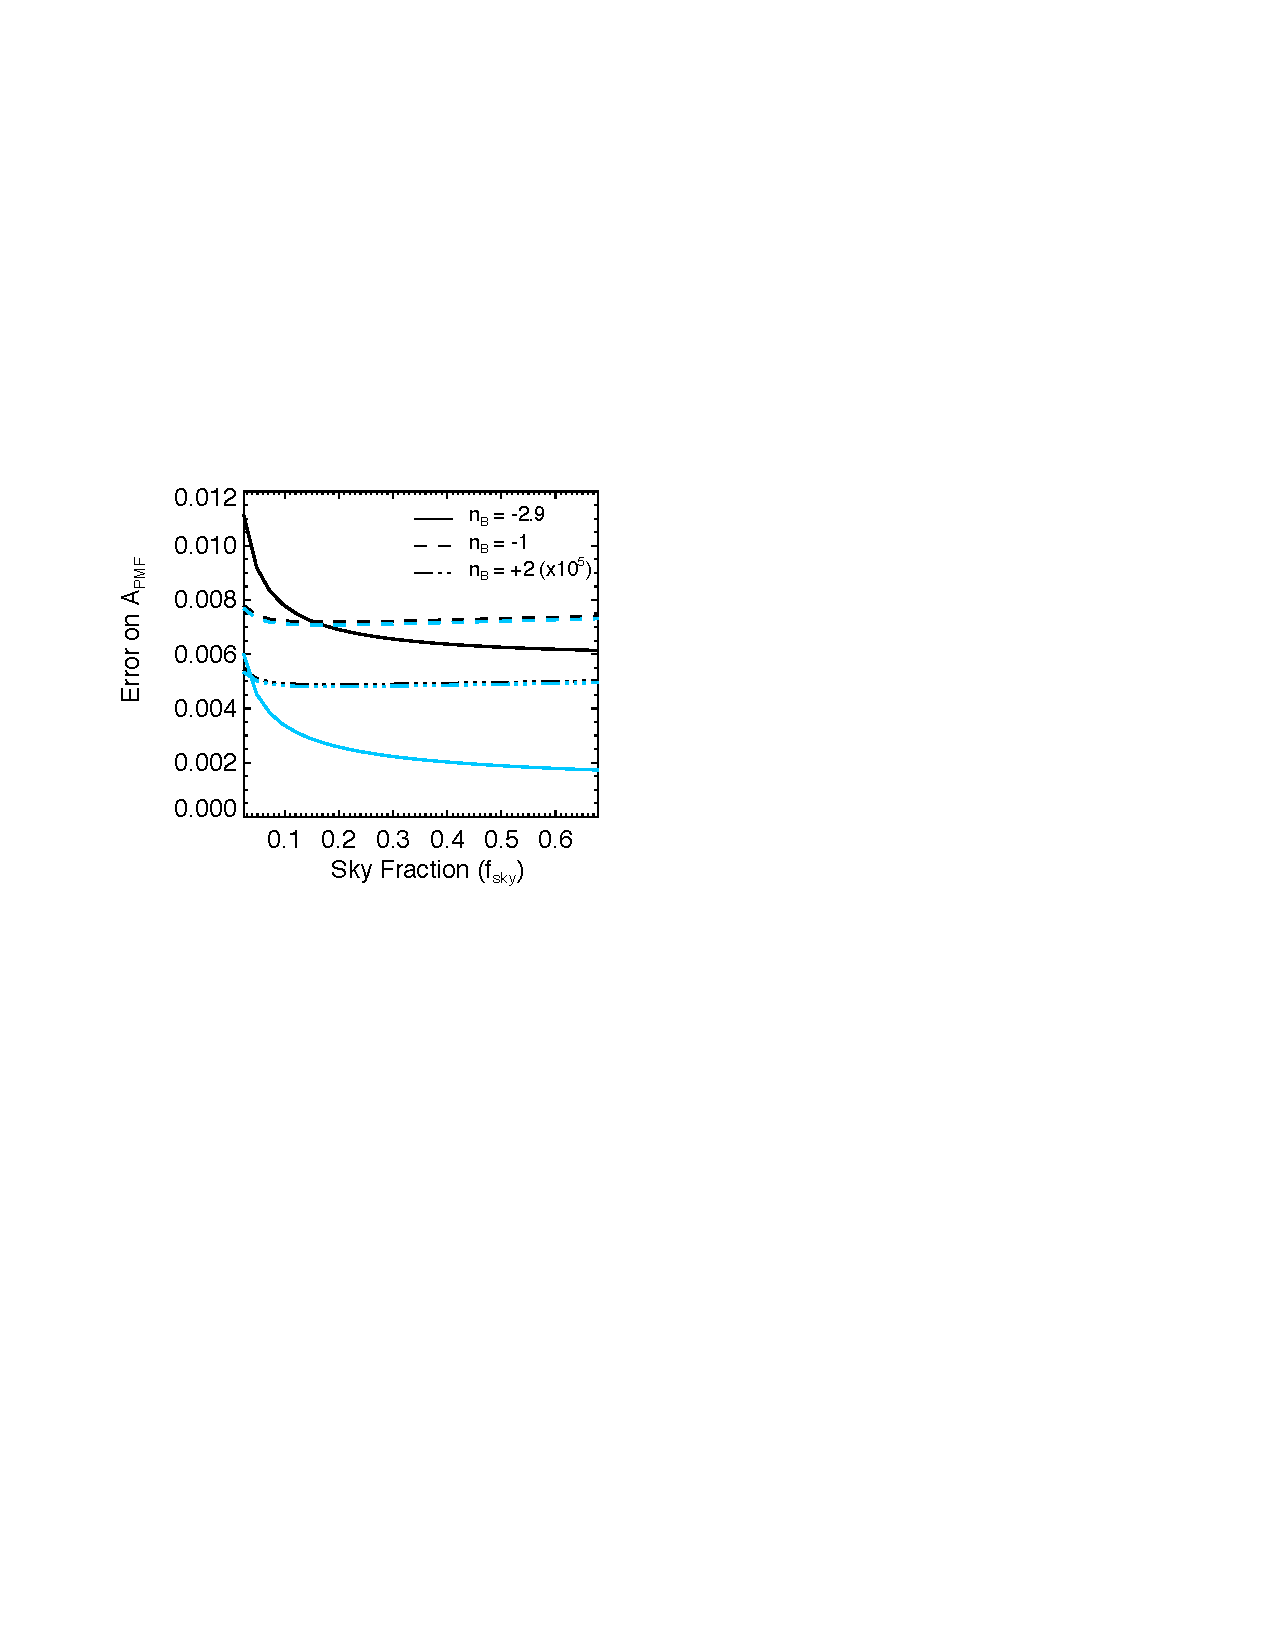
\includegraphics[width=0.45\textwidth,clip,trim={1.5cm 12.5cm 11cm 7.5cm}]{pmf_area.pdf}
  \caption[Area dependence]{
  The forecasted uncertainty on the PMF power, \apmf{}, falls as the survey area increases. 
  In particular, observing more than $\sim$\,15\% of the sky is strongly preferred for PMF searches. 
  Fortunately, the CMB-S4 survey concepts being discussed cover even larger areas of sky. 
  The black solid line shows the forecast uncertainty as a function of area in the 11-parameter cosmological model.
  The purple dot-dash line shows the same, except in the restricted \lcdm{}+\apmf{} 7-parameter model. 
  In both cases, better limits on PMFs will be achieved with wider surveys.
    \label{fig:area}
  }
\end{figure}
A third question is whether it is better to integrate deeply on a small patch of sky or observe a wide area. 
As shown in  Fig.~\ref{fig:area}, observing at least 15\% of the sky is very important to a PMF search, and it is best  to cover as much sky as possible. 
A caveat to this analysis is that it is likely easier to remove galactic foregrounds to a specified level on targeted, `clean' patches as opposed to a substantial fraction of the sky, and we would expect galactic foregrounds to be important for the large angular scales. 
With that said, the PMF constraints improve by a factor of 1.4-1.5 (depending on the cosmological model) going from 10\% to 25\% of the full sky, and improve by another factor of 1.4-1.5 by going to the 70\% of the sky (the widest area likely to be possible after galactic cuts).


Finally, we consider if searches for PMFs introduce new requirements on the accuracy to which the instrumental beam or overall calibration of an experiment must be known. 
We parameterize the beam uncertainty as a fractional uncertainty on the FWHM of the Gaussian beam, and calibration uncertainty as an overall power uncertainty. 
We find negligible, sub-percent shifts in the forecasted uncertainty for calibration uncertainties from 0.2 to 5\% and beam FWHM uncertainties from 2 to 12.5\%. 
The PMF constraints are insensitive to the beam and calibration uncertainties. 

\section{Conclusions}
\label{sec:conclusions}

In this work, we have improved the current upper limits on the strength of any primordial magnetic fields by including more CMB B-mode polarization data. 
By adding \bicepkeck{}, \pb, and \sptpol{} to \planck{} we find the 95\% CL upper limit on the PMF power falls from $\apmf < 0.73$ to $\apmf < 0.35$. 
The biggest contributor to this improvement is the low-$\ell$ data from \bicepkeck{}. 

We have also shown that the next generation of experiments should dramatically reduce these limits, and potentially detect PMFs for the first time. 
These so-called stage III experiments, which will begin taking data in 2017, expect to set upper limits at the level of $\apmf < 0.0062$ even after marginalizing over a five-parameter extension to \lcdm.

The potential for detection increases even further with planned experiments like the Simons Observatory or CMB-S4. 
We show that an ideal version of CMB-S4 might decrease the 95\% CL upper limits eight-fold, to $\apmf < 0.0008$, and even non-ideal versions can easily set upper limits on order of $\apmf < 0.001$, i.e.~ a six-fold improvement over the forecasts for the stage III experiments and a 330-fold improvement over the current limits. 
These experiments will be very exciting probes of PMFs and other sources of cosmic birefringence. 

\acknowledgments

We thank Srinivasan Raghunathan and Federico Bianchini for valuable feedback on the manuscript. 
C. Reichardt is the recipient of an Australian Research Council Future Fellowship (FT150100074), and also acknowledges support from the University of Melbourne. 
CF acknowledges support from NASA grants NASA NNX16AJ69G and NASA NNX16AF39G. 
This research used resources of the National Energy Research Scientific Computing Center, which is supported by the Office of Science of the U.S. Department of Energy under Contract No. DE-AC02-05CH11231. 
We acknowledge the use of the Legacy Archive for Microwave Background Data Analysis (LAMBDA). Support for LAMBDA is provided by the NASA Office of Space Science.


\bibliography{pmf}


\end{document}
